%!TEX root = ../../dissertacao.tex
\label{chap:sec-protocols}
This chapter surveys the main aspects of security protocols, explaining its common properties, goals, and frequent attacks methods. A basic notation, which will be used along all this document, will be presented as well.





\section{Basic Notions}
Security protocols are handy tools for providing protection among communication protocols and systems. They can be informally defined as a set of steps executed between multiple entities, aiming to ensure a reliable and secure communication between them. Current protocol specifications vary in quality, purpose and syntax, although they are the base documents for formally reasoning about these protocols \cite{Abadi99}. More definitions on security protocols can be obtained at \cite{BoydMathuria2008} and \cite{RyanSchneider2010}.

As a communication agreement, security protocols are inherently concurrent, leading to a big spectrum of possibilities among its steps, peers behavior and system states. When considering the attacker factor - an agent who can both act as a legal participant or produce and inject fake information to exploit the protocol - the difficult in designing a reliable solution can grow dramatically. For the very same reason, it is difficult to design a good security protocol and easy to develop a defective one \cite{Bella2007}.

Protocol goals are subtle: they depend on the environment, resources and the protocol architecture itself. Many goals may be present as, for instance, authentication, key establishment, confidentiality, integrity, availability and others. Some of those goals may have varying definitions in the literature, like authentication \cite{Abadi99}. Nevertheless, some properties and concepts can be universal among security protocols, as well as some goals are a consensus in the literature \cite{RyanSchneider2010}.





\section{Attacker Assumptions}
A basic assumption for every entity engaged in a security protocol session is that the knowledge about the environment is uncertain. In other words, agents will interact with other participants, which can be hostile or not, and the communication channel is generally untrusted. Moreover, it is wise to expect the worse, since security properties are relative to the resource of attackers \cite{BoydMathuria2008}. It is common to provide guarantees assuming that attackers could perform unlikely achievements, like obtaining session keys or acting as a legal peer. This can improve the system resilience.

A suitable approach for attacker modeling is the classic work of Dolev-Yao \cite{DolevYao81}. In this model, the attacker is described in a general way, giving her full control of the network and protocol operation. Therefore, it is interesting to model her capabilities in the following assumptions, based on \cite{BoydMathuria2008}:

\begin{enumerate}
  \item The adversary is able to eavesdrop on all messages sent on the network;
  \item The adversary is able to alter any message captured during protocols sessions, using any information available. Also, it can re-route to other peers and create new messages at any time;
  \item The adversary may be a legal participant, an outsider or both;
  \item The adversary can decipher or obtain information from a current session combining pieces of data from previous sessions.
\end{enumerate}





\section{Cryptography and Key Management}
Despite being a crucial basis on the success of a reliable protocol, cryptography will be treated in an abstract way here, since what matters are its concepts and its impact on the protocol behavior. Cryptographic keys are the basis for generating a secure communication, where it is used for enciphering all data transmitted along the channels. However, creating a valid new session key demands a previous secured channel. Indeed, the establishment of such key may occur in one of these three contexts:

\begin{enumerate}
  \item The peers have a pre-shared key, already created;
  \item An off-line public infrastructure may be used, where the participants hold certified public keys;
  \item An on-line public infrastructure may be used, where peers share a key with a trusted third-party entity.
\end{enumerate}

Concerning the user entity and based on these concepts, the generation of session keys can be based on a \textit{key transport} or \textit{key agreement} protocol. The first is associated with protocols where participants use on-line servers, which generates keys and transfers them to users. The second is often associated with the off-line infrastructures, which generates the key based on inputs provided by the peers. Hybrid protocols for key generation based on these two approaches also exist \cite{BoydMathuria2008}.





\section{Notation}
Through this document, we will need a consistent notation for expressing protocol actions and symbols. We will use a system based on the one presented in \cite{Bella2007}, which brings aspects from the seminal work of \cite{Burrows90}, since it is our main reference method for verification in this work.

Primitive data instances, such messages, timestamps and \textit{nounces} can be represented as simple mnemonic letters and the encryption of such entities are represented with subscripts, for example, a message $M$ using a key $K$ is represented by $M_K$. When giving authorship to a given resource, we also use subscripts, such a key from agent $A$ resulting in the symbol $K_A$. Accordingly, the session key established between agents $A$ and $B$ is represented by the symbol $K_{AB}$. On further examples or proofs, the definitions will be straightforward.

Concerning the key scope, a distinction is also required. For that, private keys are preceded by the indicator $s$, meaning signature, and public keys are preceded by $p$, meaning public. Hence, the private and public keys of peer $A$ would be represented as $sK_A$ and $pK_A$, respectively.

Besides, the use of fat brackets ($\lBrack$ and $\rBrack$) has two purposes: it can distinguishes protocol messages from sets and represents a concatenation. Therefore, a concatenation of messages $m$ and $n$ is represented as $\Bracks{m,n}$ and its encryption under key $K$ is written as $\Bracks{m,n}_K$.

Finally, we need to represent message transportation. The syntax follows a simple structure, where each protocol step is represented in one line, following the order: step number, sender, recipient and finally the message contents, which contains at least one symbol. For instance, we use the hypothetic protocol provided in Figure \ref{prt:notation-example}, where the host $A$ sends its identity and a nonce $N_A$ to a host $B$, who replies with the nonce and a fresh session key $K_{AB}$, both encrypted under its private signature key $K_B$.

\begin{figure}[ht]
  \centering
    \[
    \begin{array}{rlcl}
      1. & A \longrightarrow B &:& A, N_A \\
      2. & B \longrightarrow A &:& \Bracks{N_A, K_{AB}}_{K_B} \\
    \end{array}
    \]
  \caption{Example protocol for notation undestanding}
  \label{prt:notation-example}
\end{figure}

As a background example intended to provide a better understanding of the next concepts, the problems within some protocol designs and the syntax presented in this section, we describe a common situation, where two agents, $A$ and $B$ (commonly called Alice and Bob), wants to communicate securely. For that, they generate a session key $K_{AB}$, aided by a trusted third-party peer, the Server $S$. Such key will be used for ciphering future messages, so it must be newly generated and only known to these three entities.

In Figure \ref{prt:naive-session-key}, a protocol is designed as first and naive attempt to represent this situation. At first, Alice sends to the server her and Bob identities, who intend to communicate with each other. The Server replies to her the session key $K_{AB}$, who Alice readily forwards to Bob, along with her identity. Over the next sections, we will identify problems and redesign the protocol.

\begin{figure}[ht]
  \centering
  \[
    \begin{array}{rlcl}
      1. & A \longrightarrow S & : & A, B \\
      2. & S \longrightarrow A & : & K_{AB} \\
      3. & A \longrightarrow B & : & K_{AB}, A \\
    \end{array}
  \]
  \caption{Naive session key establishment}
  \label{prt:naive-session-key}
\end{figure}





\section{Confidentiality}
Confidentiality (or secrecy) is a required aspect when systems should not leak information to untrusted peers, guaranteeing access only for the trusted ones. Also, it is one of the most required properties among security protocols. As seem previously, cryptography is a suitable method for generating keys used for securing messages. We define a encryption scheme consisting of a key set $\mathcal{K}$, a message set $\mathcal{M}$ and a ciphertext set $\mathcal{C}$ and three main algorithms:

\begin{itemize}
  \item \textbf{Key Generation:} outputing an encryption key $K \in \mathcal{K}$ and decryption key $K^{-1} \in \mathcal{K}$;

  \item \textbf{Encryption:} taking a message $m \in \mathcal{M}$ and encryption key $K \in \mathcal{K}$, it outputs the ciphertext $c \in \mathcal{C}$, which is defined as $c = m_K$;

  \item \textbf{Decryption:} taking a ciphertext $c \in \mathcal{C}$ and decryption key $K^{-1} \in \mathcal{K}$, it outputs the message $m \in \mathcal{M}$, which is defined as $m = D_{K^{-1}}(c)$.
\end{itemize}

Considering key properties, when a given encryption key $K$ is the same as the decryption key $K^{-1}$, e.g.\ $K = K^{-1}$, it is stated that they are \emph{symmetric} keys. Otherwise, they are \emph{non-symmetric} keys, normally engaged in a process of public key encryption, commonly used nowadays \cite{RyanSchneider2010}.

Secrecy consistency can be discussed with respect to some degree of flexibility. An active spy should not be able to learn something on generated ciphertexts. The property of \textit{semantic security} states that if an attacker can compute something from a ciphertext, it must also be able to compute it from its equivalent message. Stronger than that, \textit{non-malleability} makes impossible to transform a given ciphertext in a related one without knowing the input plaintext. A detailed discussion on this topic is provided in \cite{Abadi99}.

Considering our previously presented example, it is easy to state that confidentiality is compromised in the protocol. The session key $K_{AB}$ is transmitted in cleartext over the network, so an active spy could simply extract it from the channel and use it for decipher subsequent messages exchanged between $A$ and $B$.

We redesign our first attempt, given in Figure~\ref{prt:session-key-confidentiality}. Here, we define keys $K_{AS}$ and $K_{BS}$ as previously shared keys known by the server and agents $A$ and $B$, respectively. Alice will repeat the first step of the former protocol, but now the server will reply with a tuple, composed by the session key $K_{AB}$ encrypted with shared keys $K_{AS}$ and $K_{BS}$. Finally, Alice sends the session key, encrypted with Bob shared key, and her identity to Bob.

\begin{figure}[ht]
  \centering
  \[
    \begin{array}{rlcl}
      1. & A \longrightarrow S &:& A, B \\
      2. & S \longrightarrow A &:& \Bracks{K_{AB}}_{K_{AS}}, \Bracks{K_{AB}}_{K_{BS}} \\
      3. & A \longrightarrow B &:& \Bracks{K_{AB}}_{K_{BS}},A \\
    \end{array}
  \]
  \caption{Session key establishment with proper confidentiality}
  \label{prt:session-key-confidentiality}
\end{figure}

If the agents are not compromised, then the spy cannot retrieve the session key $K_{AB}$, since she does not know the shared keys from $A$ and $B$. Consequently, the communication between Alice and Bob is protected.





\section{Authentication}
\label{sec:protocols:auth}
Authentication is a vastly studied topic among security researchers, since its definition is not really well-established, causing problems for a correct implementation of this property among protocols. Such topic is well discussed in \cite{Gollmann2000}.

Here, we recall some definitions provided in \cite{Diffie92} and \cite{RyanSchneider2010}. Authentication can be defined as the oath on a communication session where peers can be assured about each others identity. Similarly, the establishment of trust in a peer identity, can be related to the generation of a session key for further communication among the peers involved in the session, validating each message.

Concerning the authentication of origin, confirming the authorship of $A$ of a given message received by $B$, in a given protocol session, gives some guarantees. The first one is that $A$ is alive and she must have sent the message. Further, a stronger property claims that she truly intended to communicate with $B$, agreeing in following the protocol directives.

Thus, the received message must not get altered in any way. This assurance implies the property of \textbf{integrity}, which means that no message can be corrupted along its way to the recipient. For this reason, authentication and integrity are commonly associated into a single property. Ensuring such feature may be achieved by the use of manipulation detection codes (MDC) or message authentication codes (MAC) \cite{ross-security}.

Other stronger properties may be needed. One is the pledge of the received message to be the first and original one, avoiding the acceptance of repeated messages. Concerning the protocol which will be studied in Chapter \ref{chap:dap}, this notion is crucial. A good discussion on this is also given in \cite{Gollmann2000}.

Now we focus on our working example. As stated, the attacker can intercept and modify messages, since it has full control of the network. We consider two situations, presented in Figures~\ref{fig:auth-attack1} and \ref{fig:auth-attack2}.

\begin{figure}[ht]
  \centering
  \begin{tikzpicture}
    \tikzstyle{node}=[circle,draw,thick,inner sep=4mm,minimum size=4mm]
      \node (S) at (-2, 5) [node ]{S};
      \node (A) at (-7, 0) [node] {A};
      \node (B) at (7, 0)  [node] {B};
      \node (E) at (0, 0)  [node] {E};

      \path[->,draw] (A) edge [sloped,above,bend left] node {1. $A, B$} (S);

      \draw[->] (S) -- (A) node[midway,auto] {2. $\{K_{AB}\}_{K_{AS}}, \{K_{AB}\}_{K_{BS}}$};
      \draw[->] (A) -- (E) node[midway,auto] {3. $\{K_{AB}\}_{K_{BS}}, A$};
      \draw[->] (E) -- (B) node[midway,auto] {4. $\{K_{AB}\}_{K_{BS}}, X$};
  \end{tikzpicture}
  \caption{First attack possibility against Protocol \ref{prt:session-key-auth}}
  \label{fig:auth-attack1}
\end{figure}

In the first case, the Spy intercepts the message containing the session key and $A$'s identity, replacing $A$'s identity for another identity $X$, and sending it to $B$. Here, $X$ could be any agent identity, including the spy itself, and the security failure consists exactly in the fact that the guarantee of knowing who is sending a message does not hold, even though the spy does not know the session key $K_{AB}$.

The second case presents a more serious flaw. Here, the Spy intercepts the first message from $A$, replacing $B$'s identity by its own, and sends it to the server. Therefore, the server will provide a session key $K_{AE}$, destined for communication between $A$ and $E$. Additionally, the spy will also impersonate $B$, receiving the session key $K_{AE}$ and $A$'s identity, establishing a legal and ciphered communication channel with $A$. The problem here relies in the fact that $A$ supposes that such communication is being held with $B$, which is a false statement. So, not only the authentication of origin, but the session key is also compromised.

\begin{figure}[ht]
  \centering
  \begin{tikzpicture}
    \tikzstyle{node}=[circle,draw,thick,inner sep=4mm,minimum size=4mm]
      \node (S) at (-2, 5) [node ]{S};
      \node (E) at (-7, 0) [node] {E};
      \node (E2) at (7, 0)  [node] {E};
      \node (A) at (0, 0)  [node] {A};

      \path[->,draw] (A) edge [sloped,above] node {1. $A, B$} (E);
      \path[->,draw] (E) edge [sloped,above] node {2. $A, E$} (S);
      \path[->,draw] (S) edge [sloped,above, bend right] node {3. $\{K_{AE}\}_{K_{AS}}, \{K_{AE}\}_{K_{ES}}$} (E);
      \path[->,draw] (E) edge [sloped,below, bend right] node {4. $\{K_{AE}\}_{K_{AS}}, \{K_{AE}\}_{K_{ES}}$} (A);
      \path[->,draw] (A) edge [sloped,above] node {5. $\{K_{AE}\}_{K_{ES}}, A$} (E2);
  \end{tikzpicture}

  \caption{Second attack possibility against Protocol \ref{prt:session-key-auth}}
  \label{fig:auth-attack2}
\end{figure}

We rewrite our approach, redefining the protocol, which is given in Figure~\ref{prt:session-key-auth}. Now, the session key is linked with the identity of its owners, since the server replies Alice with two tuples: the session key and the identity of the participants, encrypted with their shared key. At the end, Alice forwards her identity, together with $K_{AB}$, to $B$. Note that now, the spy cannot replace any identity, since it is also encrypted and thus, authentication is preserved.

\begin{figure}[ht]
  \centering
  \[
    \begin{array}{rlcl}
      1. & A \longrightarrow S &:& A, B \\
      2. & S \longrightarrow A &:& \Bracks{K_{AB}, B}_{K_{AS}}, \Bracks{K_{AB}, A}_{K_{BS}} \\
      3. & A \longrightarrow B &:& \Bracks{K_{AB}, A}_{K_{BS}} \\
    \end{array}
  \]
  \caption{Session key establishment with proper confidentiality and authenticity}
  \label{prt:session-key-auth}
\end{figure}





\section{Other Goals}
In the previous section we have presented the two most desirable goals in security protocols, but it is important to mention other properties that are also cited in literature. In the following, we give brief descriptions of such properties. We opted for a non-exhaustive description, as those properties are more loosely used among protocols, even though their importance is uprising.

\textbf{Non-repudiation} is the ability of providing evidence on peers actions. Such quality differs on authentication, where the former tries to provide a identity assurance to the system and the latter produces a formal and enduring proof of authorship on actions and messages, which can be check by participants and third-parties. Consequently, the author cannot try to deny such actions. Notice that non-repudiation acts like a defense against not only outsiders, but from legitimate users as well.

\textbf{Unicity} or \textbf{freshness} is a protection against replay attacks, by providing a way to state that a message or key is new and not a replayed one from previous sessions. It is a common protocol requirement, since attacks that take advantage on old messages are increasing. At the end of this section, we will extend our working example for providing freshness of the keys.

Even if it is not the focus of this work, \textbf{availability} is considered as a desired goal in protocols, since it is crucial for systems properly maintain ongoing sessions. Not only keeping a peer available is important, but guaranteeing a session key or message reception is also a concern. Thus, modeling the attacker ability of killing protocol messages and reliable defenses against denial of service attacks is a valid concern among protocol designers.

Based on common errors found in published protocols, the work in \cite{AbadiNeedham96} presents interesting guidelines for designing reliable security protocols. Although these guidelines are not sufficient for building correctness, the document offers examples of protocols that do not follow the displayed principles and fails to fulfill its goals, arguing that such principles are indeed a convenient starting point for formulating protocols.

\begin{figure}[!ht]
  \centering
  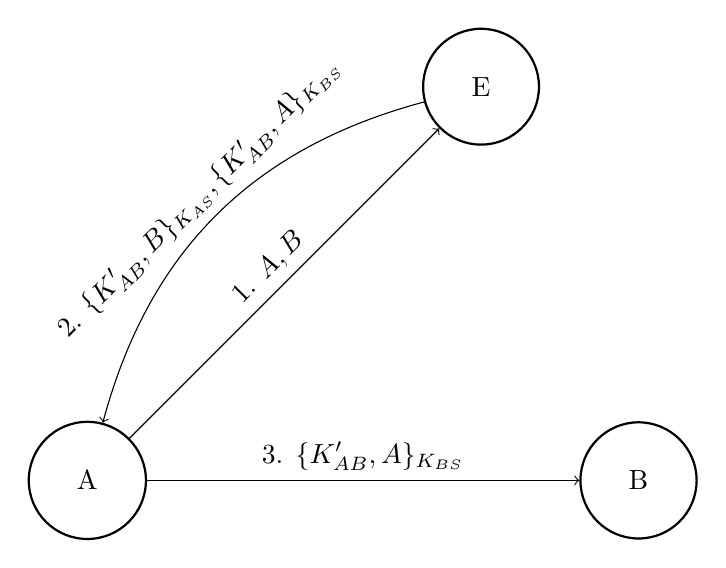
\begin{tikzpicture}
    \tikzstyle{node}=[circle,draw,thick,inner sep=4mm,minimum size=4mm]
      \node (E) at (-2, 5) [node ]{E};
      \node (A) at (-7, 0) [node] {A};
      \node (B) at (0, 0)  [node] {B};

      \path[->,draw] (A) edge [sloped,above] node {1. $A, B$} (E);
      \path[->,draw] (E) edge [sloped,above, bend right] node {2. $\{K'_{AB}, B\}_{K_{AS}}, \{K'_{AB}, A\}_{K_{BS}}$} (A);
      \path[->,draw] (A) edge [sloped,above] node {3. $\{K'_{AB}, A\}_{K_{BS}}$} (B);
  \end{tikzpicture}

  \caption{A replay attack on the protocol described on Figure \ref{prt:session-key-auth}. Key $K'_{AB}$ is obtained by the Spy from by eavesdropping previous protocol runs}
  \label{fig:attack-ex-replay}
\end{figure}

We now do a final analysis over the working example, considering the freshness property. A possible attack, extracted from \cite{BoydMathuria2008}, is represented in Figure \ref{fig:attack-ex-replay}, where the Spy impersonates the server and follow the protocol structure, but instead of using a new session key $K_{AB}$, she uses an old $K'_{AB}$ key, used in past protocol runs. Even if the spy does not know the value of $K'_{AB}$, she can replay previous messages encrypted with $K'_{AB}$ and gather more data for post cryptanalysis.

An attempt for fixing such flaw is the classical protocol of Needham-Schroeder \cite{NeedhamSchroeder78}, which uses nonces, ciphered with shared keys, for guaranteeing freshness of the session key. However, this approach was proven to contain failures \cite{Lowe96}. That said, we will focus on a reliable solution, also described in \cite{BoydMathuria2008} and illustrated in Figure~\ref{prt:session-key-complete}.

\begin{figure}[ht]
  \centering
  \[
    \begin{array}{rlcl}
      1. & B \longrightarrow A &:& B, N_B \\
      2. & A \longrightarrow S &:& A, B, N_A, N_B \\
      3. & S \longrightarrow A &:& \Bracks{K_{AB}, B, N_A}_{K_{AS}}, \Bracks{K_{AB}, A, N_B}_{K_{BS}} \\
      4. & A \longrightarrow B &:& \Bracks{K_{AB}, A, N_B}_{K_{BS}} \\
    \end{array}
  \]
  \caption{Session key establishment with proper confidentiality, authenticity and freshness}
  \label{prt:session-key-complete}
\end{figure}

The solution relies in two fresh nonces, $N_A$ and $N_B$. Now, $B$ will start the protocol, sending her identity and nonce to $A$. $A$ sends hers and $B$'s identities and nonces to the Server, who responds $A$ with $K_{AB}$, $B$ identity and $N_A$ encrypted with $A$'s shared key with the Server and an equivalent instance, encrypted with $B$'s shared key $K_{BS}$. Finally, Alice sends $B$'s instance to her, properly distributing the session key $K_{AB}$. The nonces allows the agents to check freshness of messages and its contents, the keys protect the integrity of data exchanged among peers, and the protocol is sound.





\section{Attack Approaches}
Complementing the notes on security protocols, it is interesting to provide a section about the classical and most common attack approaches studied in the literature, aiming in understanding how such threats scaled up. A non-exhaustive list, adapted from \cite{BoydMathuria2008}, is presented in Table \ref{protocol-attacks}, introducing its names and a brief explanation of its strategy.

It is essential to note that this list is not a complete guide, but an attempt to picture the mainstream on attack methods. Many attacks against systems and protocols involves combinations of several of these approaches and not all of them are applicable to all protocols. Different protocols have different purposes, therefore, the strategies for attacking them may vary.

\begin{table}
  \caption{Common types of protocols attacks}
  \label{protocol-attacks}

  {\def\arraystretch{1.5}
  \begin{tabular}[c]{l p{10cm}}
    \hline
    \textbf{Eavesdropping} & The adversary capture the data sent in the protocol \\
    \textbf{Modification} & The adversary alters the data sent in the protocol \\
    \textbf{Replay} & The adversary record data seen in previous protocol sessions and reuses it in a different, usually later, session for exploitation \\
    \textbf{Preplay} & The adversary engages in a run of the procotol prior to a run by the legitimate principals \\
    \textbf{Reflection} & The adversary sends protocol messages back to the principal who sent them \\
    \textbf{Denial of Service} & The adversary prevents or hinders legitimate messages or principals from completing the protocol \\
    \textbf{Typing Attacks} & The adversary replaces a protocol message fields of on type with a message field of another type \\
    \textbf{Cryptanalysis} & The adversary gains some useful leverage from the protocol to help in cryptanalysis \\
    \textbf{Certificate Modification} & The adversary chooses or modifies certificate data to attack one or more protocol runs \\
    \textbf{Protocol Interaction} & The adversary chooses a new protocol to interact with a known protocol \\
    \hline
  \end{tabular}
  }

\end{table}
